\documentclass[a4paper,11pt]{article}
\usepackage[verbose,a4paper,tmargin=2cm,bmargin=2cm,lmargin=2.5cm,rmargin=2.5cm]{geometry}
\usepackage[utf8]{inputenc}
\usepackage{polski}
\usepackage{amsmath}
\usepackage{amsfonts}
\usepackage{amssymb}
\usepackage{lastpage}
\usepackage{indentfirst}
\usepackage{verbatim}
\usepackage{graphicx}
\usepackage{fancyhdr}
\usepackage{listings}
\usepackage{hyperref} 
\usepackage{xcolor}
\usepackage{tikz}
\usepackage{graphicx} 
\frenchspacing
\pagestyle{fancyplain}
\fancyhf{}
\renewcommand{\headrulewidth}{0pt}
\renewcommand{\footrulewidth}{0.4pt}
\newcommand{\degree}{\ensuremath{^{\circ}}} 
\fancyfoot[L]{PSI: Justyna Hubert i Karol Podlewski}
\fancyfoot[R]{\thepage\ / \pageref{LastPage}}


\begin{document}

\begin{titlepage}
\begin{center}
\begin{tabular}{rl}
\begin{tabular}{|r|}
\hline \\
\large{\underline{210200~~~~~~~~~~~~~~~~~~~~~~~~~~~~~~~~~~~~~~~~~~} }\\
$^{numer\ indeksu}$\\
\large {\underline{Justyna Hubert~~~~~~~~~~~~~~~~~~~~~~~~~~~~~~} }\\
$^{imie\ i\ nazwisko}$ \\\\ \hline
\end{tabular} 
&
\begin{tabular}{|r|}
\hline \\
\large{\underline{210294~~~~~~~~~~~~~~~~~~~~~~~~~~~~~~~~~~~~~~~~~~} }\\
$^{numer\ indeksu}$\\
\large {\underline{Karol Podlewski~~~~~~~~~~~~~~~~~~~~~~~~~~~~~~} }\\
$^{imie\ i\ nazwisko}$ \\\\ \hline
\end{tabular} 

\end{tabular}
~\\~\\~\\ 
\end{center}
\begin{tabular}{ll}
\LARGE{\textbf{Data}}& \LARGE{2018-10-12}\\
\LARGE{\textbf{Kierunek}}& \LARGE{Informatyka}\\
\LARGE{\textbf{Rok akademicki}}& \LARGE{2018/19} \\
\LARGE{\textbf{Semestr}}& \LARGE{5} \\
\LARGE{\textbf{Specjalizacja}}& \LARGE{IOAD} \\
\LARGE{\textbf{Grupa dziekańska}}& \LARGE{3} \\\\\\\\\\
\end{tabular}

\begin{center}
\textbf{\LARGE{\\~\\Projektowanie Systemów\\Informatycznych\\~\\~\\}}
\end{center}


\begin{center}
\textbf{\Huge{Internetowy sklep z odzieżą:\\~\\ WearIT}} \\~\\
\end{center}

\end{titlepage}
\setcounter{page}{2}

\section {Wprowadzenie}

\subsection {Cel dokumentu}
Celem dokumentu jest przedstawienie projektu systemu informatycznego dla internetowego sklepu z odzieżą WearIT. Dokument ten prezentuje wymagania dotyczące oprogramowania, czyli opisuje funkcjonalność budowanego oprogramowania i warunki, jakie ono musi spełniać. 

\subsection {Zakres produktu}
Projektowany system będzie odpowiedzialny za obsługę składanych zamówień internetowych. Ma on za zadanie usprawnić przebieg pracy pracowników firmy zajmującej się sprzedażą odzieży oraz zautomatyzować proces handlu elektronicznego.


\section {Wymagania}

\subsection {Funkcjonalne}
\begin{itemize}
	\item Rejestracja (tworzenie konta) (możliwość rejestracji za pomocą portali społecznościowych, tj. Facebook, Google).
	\item Logowanie, wylogowywanie.
	\item Dodawanie i usuwanie produktu do koszyka.
	\item Zakup produktów znajdujących się w koszyku.
	\item Sprawdzenie dostępności produktu .
	\item Wyszukiwanie produktów według kategorii, ceny (minimalna, maksymalna), marki, rozmiaru, płci, koloru, kolekcji, stanu (przecenione, nieprzecenione).
	\item Sortowanie listy produktów w kolejności rosnącej i malejącej według ceny, popularności, trafności, daty wydania kolekcji.
	\item Formularz kontaktowy.
	\item Obsługę reklamacji, zwrotów.
	\item Organizację akcji promocyjnych.
	\item Wprowadzanie towaru do systemu.
	\item Zarządzanie stanami magazynowymi.
	\item Przygotowywanie produktów do wysyłki.
\end{itemize} 

\subsection {Niefunkcjonalne}
\begin{itemize}
	\item Certyfikat bezpieczeństwa na stronie internetowej.
	\item Obsługa baz danych.
	\item Wymagane stałe połączenie sieciowe.
	\item Długość nieaktywnej sesji.
	\item Zakupy możliwe tylko po zalogowaniu.
	\item Dodanie do koszyka produktów możliwe także dla klientów niezarejestrowanych/niezalogowanych.
	\item Dostępność systemu dla klientów na urządzeniach moblinych
	\item Maksymalna liczba produktów w koszyku to 25.
	\item Nie można dodać do koszyka produktów niedostępnych.
	\item Darmowa dostawa powyżej 300zł.
\end{itemize}

\subsection {Diagram przypadków użycia}


\section {Hierarchiczny model funkcji systemu informatycznego}
\subsection {Diagram hierarchii funkcji.}
\begin{figure}[h]
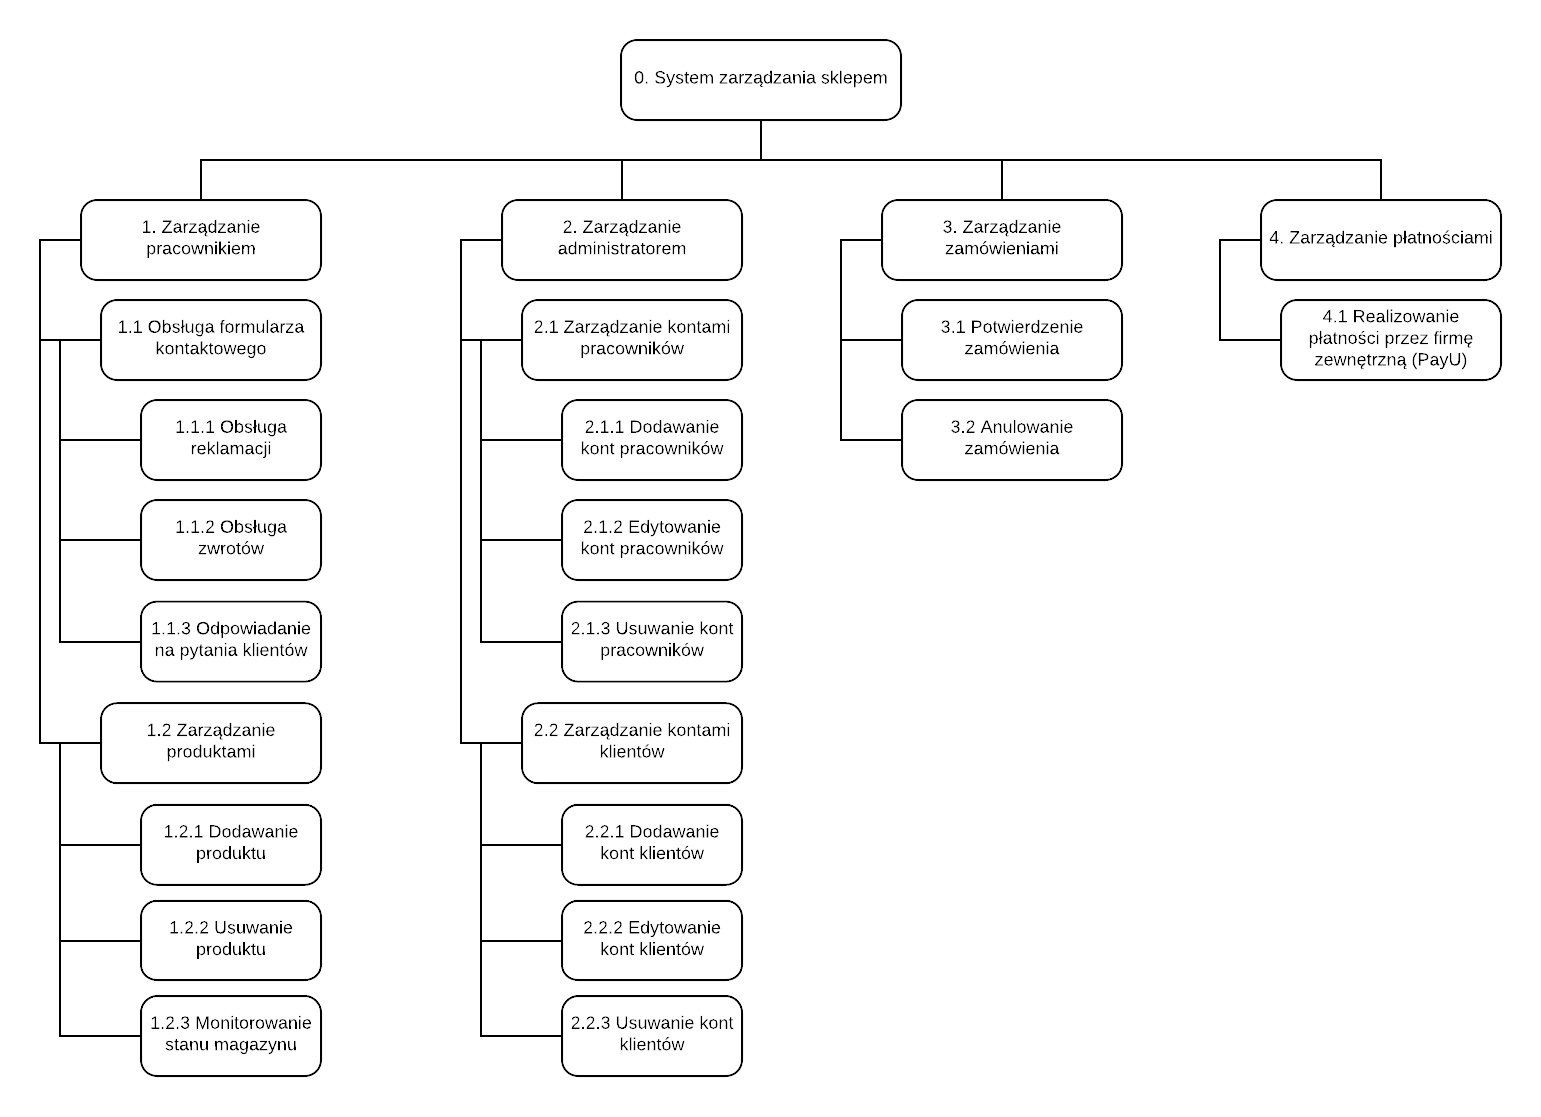
\includegraphics[width=16cm]{Diagramy/HierarchiiFunkcji.png}
\caption{Diagram hierarchii funkcji}
\end{figure}

\end{document}